% Modeled after sample-sigplan.tex
\documentclass[sigplan,anonymous,review,10pt]{acmart}
%\documentclass[sigplan,10pt]{acmart}
%% \BibTeX command to typeset BibTeX logo in the docs
\AtBeginDocument{%
  \providecommand\BibTeX{{%
    Bib\TeX}}}
\setcopyright{acmlicensed}
\copyrightyear{2018}
\acmYear{2018}
\acmDOI{XXXXXXX.XXXXXXX}
%% These commands are for a PROCEEDINGS abstract or paper.
\acmConference[Onward!]{Onward!}{Oct.\ 20-25, 2024}{Pasadena, CA}
\acmISBN{978-1-4503-XXXX-X/18/06}
% ============================================================
% ============================================================
\usepackage{xspace}
\usepackage{graphicx}
\graphicspath{{figures/}}
% ============================================================
%% Uncomment the next few lines to get sf url links:
%\usepackage{url}            
%\makeatletter
%\def\url@leostyle{%
%  \@ifundefined{selectfont}{\def\UrlFont{\sf}}{\def\UrlFont{\small\sffamily}}}
%\makeatother
%\urlstyle{leo} % Now actually use the newly defined style.
%% Choose coloured or b/w links:
%\usepackage[pdftex,colorlinks=true,pdfstartview=FitV,
% linkcolor=black,citecolor=black,urlcolor=black]{hyperref}
%\usepackage{hyperref}
\usepackage{needspace}
\newcommand{\needlines}[1]{\Needspace{#1\baselineskip}}
\usepackage{paralist}
% ============================================================
%:Markup macros for proof-reading
\usepackage{ifthen}
\usepackage[normalem]{ulem} % for \sout
\usepackage{xcolor}
\newcommand{\ra}{$\rightarrow$}
\newboolean{showedits}
\setboolean{showedits}{true} % toggle to show or hide edits
%\setboolean{showedits}{false} % toggle to show or hide edits
\ifthenelse{\boolean{showedits}}
{
	\newcommand{\meh}[1]{\textcolor{red}{\uwave{#1}}} % please rephrase
	\newcommand{\ins}[1]{\textcolor{blue}{\uline{#1}}} % please insert
	\newcommand{\del}[1]{\textcolor{red}{\sout{#1}}} % please delete
	\newcommand{\chg}[2]{\textcolor{red}{\sout{#1}}{\ra}\textcolor{blue}{\uline{#2}}} % please change
	\newcommand{\nbe}[3]{
		{\colorbox{#3}{\bfseries\sffamily\scriptsize\textcolor{white}{#1}}}
		{\textcolor{#3}{\sf\small$\blacktriangleright$\textit{#2}$\blacktriangleleft$}}}
}{
	\newcommand{\meh}[1]{#1} % please rephrase
	\newcommand{\ins}[1]{#1} % please insert
	\newcommand{\del}[1]{} % please delete
	\newcommand{\chg}[2]{#2}
	\newcommand{\nbe}[3]{}
}
%
\newcommand\rA[1]{\nbe{Reviewer A}{#1}{cyan}}
\newcommand\rB[1]{\nbe{Reviewer B}{#1}{olive}}
\newcommand\rC[1]{\nbe{Reviewer C}{#1}{magenta}}
\newcommand\ANS[1]{\nbe{Response}{#1}{teal}}

\newcommand{\THE}{\ins{the}\xspace} % "the" missing
\newcommand{\A}{\ins{a}\xspace} % "a" missing
\newcommand{\s}{\ins{s}\xspace} % "s" missing
\newcommand{\COMMA}{\ins{,}\xspace} % "," missing
\newcommand{\THAT}{\chg{which}{that}\xspace} % use "that", not "which"

% ============================================================
%:Box comments/edits
\usepackage[most]{tcolorbox}
\ifthenelse{\boolean{showedits}}
{
  \newtcolorbox{inserted}{%
       title=Inserted text:,
       colframe=blue,colback=blue!5!white,
       breakable,
       leftrule=0mm, 
       bottomrule=0mm,
       rightrule=0mm,
       toprule=0mm,
       arc=0mm, outer arc=0mm,
       oversize
  }
  \newtcolorbox{deleted}{%
       title=Deleted text:,
       colframe=red,colback=red!5!white,
       breakable,
       leftrule=0mm, 
       bottomrule=0mm,
       rightrule=0mm,
       toprule=0mm,
       arc=0mm, outer arc=0mm,
       oversize
  }
  \newtcolorbox{refactored}{%
       % title=Heavily modifed/refactored text:,
       title=Rewritten text:,
       colframe=blue,colback=red!5!white,
       breakable,
       leftrule=0mm, 
       bottomrule=0mm,
       rightrule=0mm,
       toprule=0mm,
       arc=0mm, outer arc=0mm,
       oversize
  }
}{
  \newenvironment{inserted}{}{}
  %\newenvironment{deleted}{ \begin{comment} }{ \end{comment} }
  \let\deleted\comment
  \newenvironment{refactored}{}{} 
}
% ============================================================
%:Put edit comments in a really ugly standout display
%\usepackage{ifthen}
%\usepackage{amssymb} % Avoid error: Command `\Bbbk' already defined.
\newboolean{showcomments}
\setboolean{showcomments}{true}
%\setboolean{showcomments}{false}
\newcommand{\id}[1]{$-$Id: scgPaper.tex 32478 2010-04-29 09:11:32Z oscar $-$}
\newcommand{\yellowbox}[1]{\fcolorbox{gray}{yellow}{\bfseries\sffamily\scriptsize#1}}
\newcommand{\triangles}[1]{{\sf\small$\blacktriangleright$\textit{#1}$\blacktriangleleft$}}
\ifthenelse{\boolean{showcomments}}
%{\newcommand{\nb}[2]{{\yellowbox{#1}\triangles{#2}}}
{\newcommand{\nbc}[3]{
 {\colorbox{#3}{\bfseries\sffamily\scriptsize\textcolor{white}{#1}}}
 {\textcolor{#3}{\sf\small$\blacktriangleright$\textit{#2}$\blacktriangleleft$}}}
 \newcommand{\version}{\emph{\scriptsize\id}}}
{\newcommand{\nbc}[3]{}
 \newcommand{\version}{}}
\newcommand{\nb}[2]{\nbc{#1}{#2}{orange}}
\newcommand{\here}{\yellowbox{$\Rightarrow$ CONTINUE HERE $\Leftarrow$}}
\newcommand\rev[2]{\nb{TODO (rev #1)}{#2}} % reviewer comments
\newcommand\fix[1]{\nb{FIX}{#1}}
\newcommand\todo[1]{\nb{TO DO}{#1}}
%\newcommand\XXX[1]{\nbc{XXX}{#1}{brown}}
%\newcommand\XXX[1]{\nbc{XXX}{#1}{cyan}}
%\newcommand\XXX[1]{\nbc{XXX}{#1}{darkgray}}
%\newcommand\XXX[1]{\nbc{XXX}{#1}{gray}}
%\newcommand\XXX[1]{\nbc{XXX}{#1}{magenta}}
%\newcommand\XXX[1]{\nbc{XXX}{#1}{olive}}
%\newcommand\XXX[1]{\nbc{XXX}{#1}{orange}}
%\newcommand\XXX[1]{\nbc{XXX}{#1}{purple}}
%\newcommand\XXX[1]{\nbc{XXX}{#1}{red}}
%\newcommand\XXX[1]{\nbc{XXX}{#1}{teal}}
%\newcommand\XXX[1]{\nbc{XXX}{#1}{violet}}
% ============================================================
\newboolean{isblinded}
\setboolean{isblinded}{true}
%\setboolean{isblinded}{false}
\ifthenelse{\boolean{isblinded}}
{\newcommand\blind[1]{BLINDED\xspace}}
{\newcommand\blind[1]{#1\xspace}}
% ============================================================
\newcommand{\seclabel}[1]{\label{sec:#1}}
%\newcommand{\secref}[1]{Section~\ref{sec:#1}} <- use \autoref instead!
\newcommand{\figlabel}[1]{\label{fig:#1}}
%\newcommand{\figref}[1]{Figure~\ref{fig:#1}}
\newcommand{\tablabel}[1]{\label{tab:#1}}
%\newcommand{\tabref}[1]{Table~\ref{tab:#1}}
% ============================================================
\newcommand{\ie}{\emph{i.e.},\xspace}
\newcommand{\eg}{\emph{e.g.},\xspace}
\newcommand{\etal}{\emph{et al.}\xspace}
\newcommand{\etc}{\emph{etc.}\xspace}
% ============================================================

% $Author: oscar $
% $Date: 2009-11-06 14:37:12 +0100 (Fri, 06 Nov 2009) $
% $Revision: 29604 $
%=============================================================
% ST80 listings macros
% Adapted from Squeak by Example book
%=============================================================
% If you want >>> appearing as right guillemet, you need these two lines:
%\usepackage[T1]{fontenc}
%\newcommand{\sep}{\mbox{>>}}
% Otherwise use this:
\newcommand{\sep}{\mbox{$\gg$}}
%=============================================================
%:\needlines{N} before code block to force page feed
%\usepackage{needspace}
%\newcommand{\needlines}[1]{\Needspace{#1\baselineskip}}
%=============================================================
%:Listings package configuration for ST80
\usepackage[english]{babel}
%\usepackage{amssymb,textcomp}
\usepackage{listings}
% \usepackage[usenames,dvipsnames]{color}
% \usepackage[usenames]{color}
% \definecolor{source}{gray}{0.95}
\lstdefinelanguage{Smalltalk}{
  % morekeywords={self,super,true,false,nil,thisContext, eachModel}, % This is overkill
  morestring=[d]',
  morecomment=[s]{"}{"},
  alsoletter={\#:},
  escapechar={!},
  literate=
    {BANG}{!}1
    {UNDERSCORE}{\_}1
    % {\\st}{Smalltalk}9 % convenience -- in case \st occurs in code
    % {'}{{\textquotesingle}}1 % replaced by upquote=true in \lstset
    {_}{{$\leftarrow$}}1
    {>>>}{{\sep}}1
    {^}{{$\uparrow$}}1
    {~}{{$\sim$}}1
    {-}{{\sf -\hspace{-0.13em}-}}1  % the goal is to make - the same width as +
    {+}{\raisebox{0.08ex}{+}}1		% and to raise + off the baseline to match -
    {-->}{{\quad$\longrightarrow$\quad}}3
	, % Don't forget the comma at the end!
  tabsize=4
}[keywords,comments,strings]

\definecolor{source}{gray}{0.95}

\lstset{language=Smalltalk,
	basicstyle=\sffamily,
	keywordstyle=\color{black}\bfseries,
%	numbers=left,                   % where to put the line-numbers
%	numberstyle=\footnotesize,      % the size of the fonts that are used for the line-numbers
%	stepnumber=1,                   % the step between two line-numbers. If it is 1 each line will be numbered
%	numbersep=5pt,                  % how far the line-numbers are from the code
%	stringstyle=\ttfamily, % Ugly! do we really want this? -- on
	mathescape=true,
	showstringspaces=false,
	keepspaces=true,
	breaklines=true,
	breakautoindent=true,
	backgroundcolor=\color{source},
	%lineskip={-1pt}, % Ugly hack
	upquote=true, % straight quote; requires textcomp package
	columns=fullflexible} % no fixed width fonts
% In-line code (literal)
% Normally use this for all in-line code:
\newcommand{\st}{\lstinline[mathescape=false,backgroundcolor=\color{white},basicstyle={\sffamily\upshape}]}
% In-line code (latex enabled)
% Use this only in special situations where \ct does not work
% (within section headings ...):
\newcommand{\lst}[1]{{\textsf{\textup{#1}}}}
% Code environments
\lstnewenvironment{code}{%
	\lstset{%
		% frame=lines,
		frame=single,
		framerule=0pt,
		mathescape=false
	}
}{}

% Useful to add a matching $ after code containing a $
% \def\ignoredollar#1{}
%=============================================================

% ============================================================
% Macros for this paper
%\renewcommand{\nbc}[3]{} % To hide reviewer comments
\newcommand\on[1]{\nbc{ON}{#1}{olive}} % add more author macros here
\newcommand\tg[1]{\nbc{TG}{#1}{blue}}
\newcommand\ac[1]{\nbc{AC}{#1}{teal}}
%\newcommand\XXX[1]{\nbc{XXX}{#1}{red}}
%\newcommand\XXX[1]{\nbc{XXX}{#1}{violet}}
\usepackage{caption}
\captionsetup{aboveskip=5pt,belowskip=-10pt} % Adjust the space around figure captions
%\usepackage{enumitem}
%\setlist[description]{font=\itshape}
\newcommand{\GT}{\lst{GT}\xspace} % In case we want to display it differently ...
\newcommand\lmaf{\lst{Ludo\-Move\-Assert\-ion\-Fail\-ure}\xspace}
% ============================================================
% Optionally anonymize selected names
\newboolean{anonymous}
\setboolean{anonymous}{true}
\newcommand\anonymize[2]{\ifthenelse{\boolean{anonymous}}{#2}{#1}\xspace}
\newcommand\feenk{\anonymize{feenk}{anonymous company}}
% ============================================================
\begin{document}
\title{Moldable Exceptions}
\author{Andrei Chi\c{s}}
\affiliation{%
  \institution{feenk gmbh}
  \city{Wabern}
  \country{Switzerland}}
\email{andrei.chis@feenk.com}
\author{Tudor G\^irba}
\affiliation{%
  \institution{feenk gmbh}
  \city{Wabern}
  \country{Switzerland}}
\email{tudor.girba@feenk.com}
\author{Oscar Nierstrasz}
\affiliation{%
  \institution{feenk gmbh}
  \city{Wabern}
  \country{Switzerland}}
\email{oscar.nierstrasz@feenk.com}

\renewcommand{\shortauthors}{Chi\c{s} et al.}

\begin{abstract}
Debugging is hard.
Debuggers are mostly the same.
They show you a stack, a way to sample the state of the stack, and, if the debugger is live, a way to step through execution.
The standard debugger mostly offers a clumsy, low-level interface to track down and fix bugs.
A custom debugger, such as those developed for specific application domains, offers alternative interfaces more suitable to the specific execution context of the program being debugged.
% In contrast, a ``moldable debugger'' offers alternative interfaces based on the current execution context.
% In contrast, moldable debuggers change based on the context of the stack.
Contextual debugging views and actions greatly improve our ability to reason about the current problem.
Implementing such custom debuggers, however, is non-trivial, and poses a barrier to improving the debugging experience.
% Still, creating custom debuggers is much less trivial than extending an inspector with custom views and actions.
In this paper we introduce \emph{moldable exceptions}, a lightweight mechanism to adapt a debugger's interface based on contextual information provided by a raised exception.
% In this paper, we introduce a lightweight mechanism centered around exceptions to create custom debugging views and actions: as exceptions hold the entire necessary debugging context, extending the debugger can be as easy as extending the inspector of an exception.
%Moldable exceptions offer a lightweight mechanism to adapt a moldable debugger to the specific context of the exception raised to show more useful views and actions to a developer.
We present, through a series of examples, how moldable exceptions can enhance a live programming environment.
\end{abstract}

\keywords{Exceptions, debuggers, \todo{more ...}}

%\received{20 February 2007}
%\received[revised]{12 March 2009}
%\received[accepted]{5 June 2009}

\maketitle

% ============================================================
\section{Introduction}\label{sec:intro}

In the bad old days, all debuggers were the same.
You had commands to sample the current execution state, and you had commands to step through the running code.
Nowadays we have graphical debuggers that show us the run-time stack, and offer buttons instead of commands to step through the code, but they are still all the same.
The trouble with this is that every debugging problem is different, but debuggers all show us the same thing.

There have been numerous efforts to develop custom debuggers for various application domains and domain-specific languages.
These custom debuggers provide dedicated views and actions that are tailored to a specific application context.
\todo{add a concrete example from related work}
Building a custom debugger is, however, a non-trivial task, so this doesn't happen too often.
\todo{evidence?}
An \emph{extensible} debugger (such as {\tt deet}~\cite{Hans97a}) is designed so that it can be easily extended with new graphical views and debugging operations, but these extensions still represent a significant development effort.
A \emph{moldable debugger}~\cite{Chis15c} is a special kind of extensible debugger which activates alternative debugger interfaces depending on the current execution context, however the development of these alternative debuggers is still non-trivial.

%\ac{For the abstract/introduction we could emphasise more that even if it is currently possible to have multiple custom debuggers in GT/Pharo, the extension mechanism plays an important role.
%If the cost is high, the chances that developers will do it decreases.
%Maybe a good discussion here would be the extensions for views/searches/actions.
%There the extensions mechanism is different and we created many extensions.
%But even if the debugger is extensible we have only a few custom debuggers as the effort to create one is high.
%We will still need to have standalone debuggers with a higher cost to create in some cases (for example the SmaCC debugger), but in many cases we will benefit from being able to integrate views/actions in the debugger in an easier way.}

%\ac{In a way Moldable Exceptions augments the current extension mechanism for the debugger.
%In the current extension mechanism at each step in the execution we need to determine the list of available debuggers.
%For that we have multiple debuggers registered in the system, and we ask each debugger if it wants to handle the current context or not.
%With moldable exceptions in case we have also an exception in the current context we ask that exception to provide us with a list of of debugging views and actions to add to the current debugger and a list of new debugging interfaces.}

We propose a new, lightweight mechanism, called \emph{moldable exceptions}, to dynamically adapt a moldable debugger using contextual information provided by the exception itself.
In modern, object-oriented software, it is common practice to define dedicated classes of exceptions to signal individual run-time issues.
Each exception therefore implicitly carries knowledge about the kind of issue being raised.
Moldable exceptions leverage this knowledge by associating simple views and actions to be activated by a moldable debugger when that exception is raised.

Consider the following example.
In \autoref{fig:stringComparisonSnippet} we see an assertion that compares two strings.\footnote{All the examples are written in Pharo Smalltalk, running in the open-source Glamorous Toolkit IDE. \url{https://gtoolkit.com}}
In a normal setting, this assertion will fail, yielding a standard debugger view, as we see in \autoref{fig:genericDebugger}.
It will then take some time to putter in the debugger interface to understand the specific error (the strings don't match), and why the strings don't match.
\begin{figure}[h]
  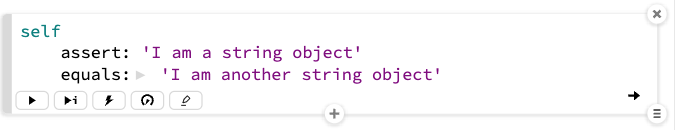
\includegraphics[width=\columnwidth]{stringComparisonSnippet}
  \caption{A failing string comparison assertion.}
  \label{fig:stringComparisonSnippet}
\end{figure}
\begin{figure}[h]
  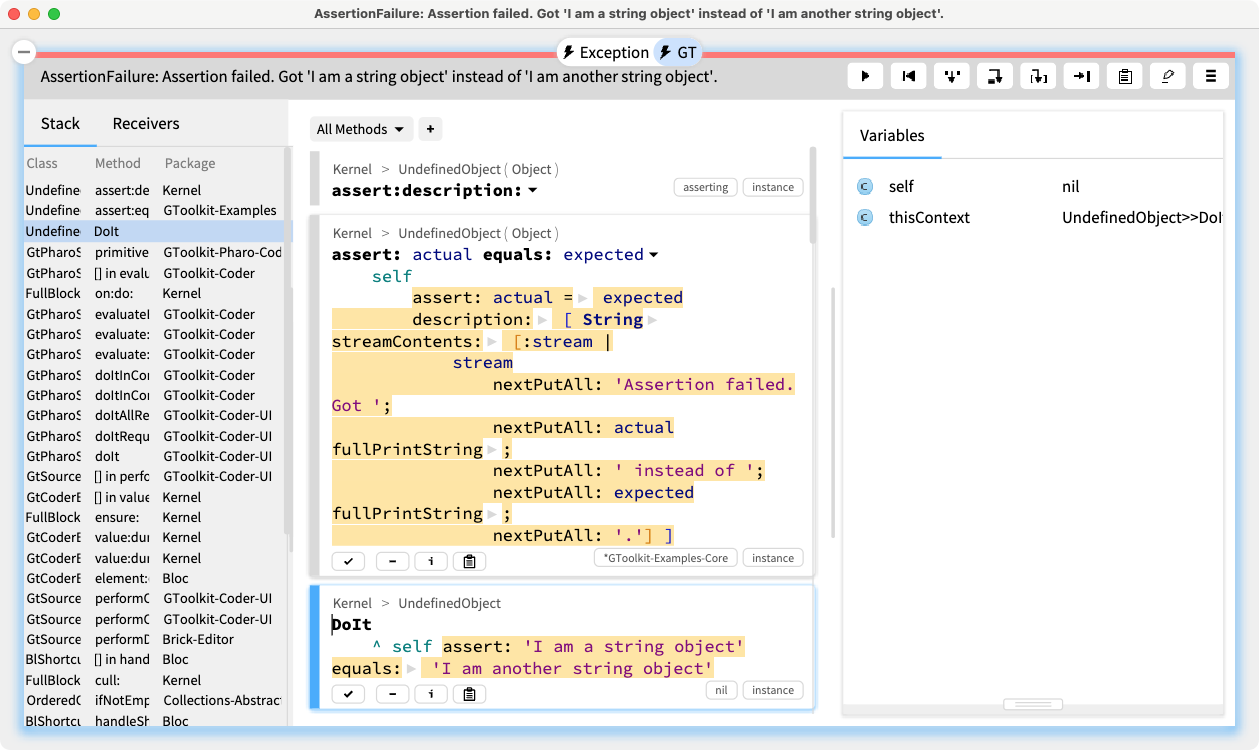
\includegraphics[width=\columnwidth]{genericDebugger}
  \caption{A generic debugger view.}
  \label{fig:genericDebugger}
\end{figure}

Suppose that instead of seeing the generic debugger, we are offered a view that highlights the actual differences, as in \autoref{fig:stringComparisonView}.
Such a view not only homes directly in on the specific problem, but also highlights the individual differences in a dedicated ``diff'' view.
Furthermore, since the diff view already exists as a component used in other applications, the development effort is close to zero.
\begin{figure}[h]
  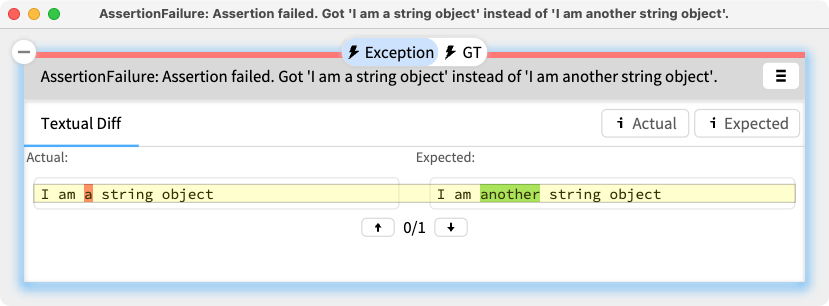
\includegraphics[width=\columnwidth]{stringComparisonView}
  \caption{A string diff debugger view.}
  \label{fig:stringComparisonView}
\end{figure}

Moldable exceptions work as follows: when an exception is raised, the exception (an object) is caught and passed to the debugger.
Every exception not only provides the debugger with the context it needs to generate the debugging UI, but it can also offer alternative views and actions.
In the case of our implementation, this is achieved by the exception class providing specially annotated debugger extension methods.

This simple mechanism allows moldable exceptions to do three things:
\begin{inparaenum}[(i)]
	\item provide domain-specific debugging views and actions,
	\item offer new debugger GUI interactions, and
	\item enable automated fixes (code transformations) for common programming errors.
\end{inparaenum}    

\todo{add section overview}
In \autoref{sec:views} we will ...
\autoref{sec:interactions}
\autoref{sec:fixes}
\autoref{sec:directions}
We discuss related work in \autoref{sec:related}.
We conclude in \autoref{sec:conclusion}.

% ============================================================
\section{Adding custom debugger views}\label{sec:views}

Moldable exceptions are instances of an Exception class that has been extended with a dedicated method for each each custom debugger view or action.
These methods are recognized by the moldable debugger through a dedicated annotation, in exactly the same way that a test runner tool in a classical IDE recognizes Java test case methods because they are tagged with a \st{@Test} annotation.

Let's go through a typical example.
Suppose we have an implementation of a Ludo\footnote{A simple game in which players move tokens around a board based on the roll of a die.
\url{https://en.wikipedia.org/wiki/Ludo}} game implemented with the help of \emph{Design by Contract}~\cite{Meye92b}.
Players alternate in throwing a die and moving a token.
Rolling a die when when a player should move, or vice versa, constitutes a precondition violation, which raises a \st{LudoMoveAssertionFailure}.
Similarly, if an attempt is made to move the wrong player's token, this will raise a precondition failure.
Normally, this would fire up the classical debugger as in \autoref{fig:ludoClassicDebugger}.
Although the precondition violation is clearly reported, the debugger interface is not ideal for tracking down the actual reason for the violation.

\begin{figure}[h]
  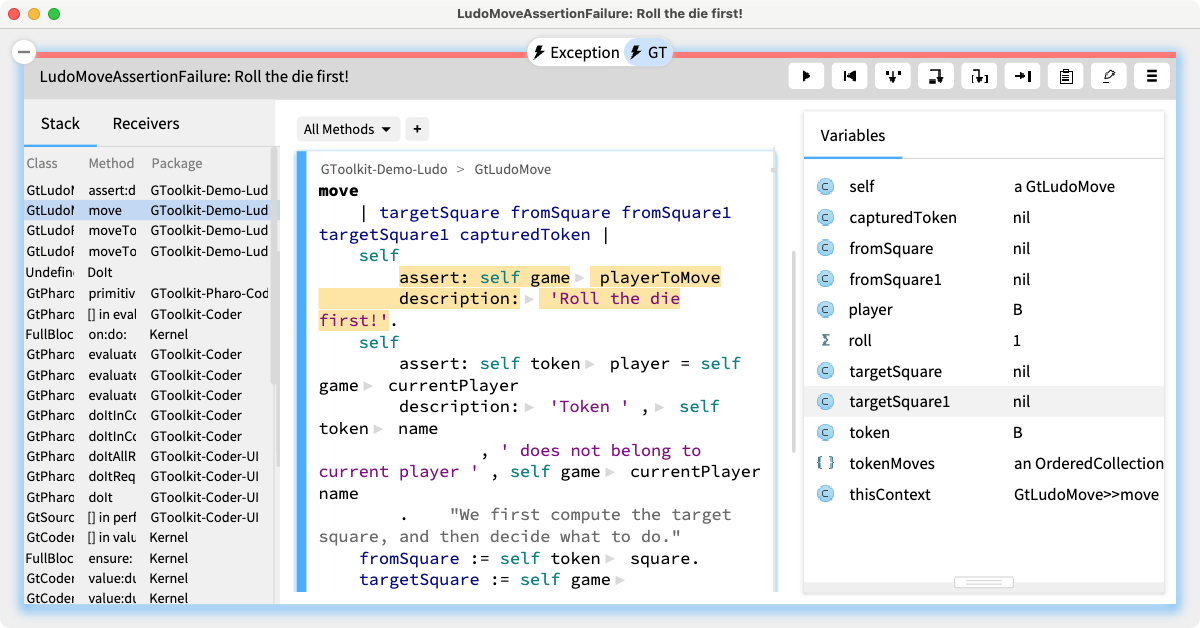
\includegraphics[width=\columnwidth]{ludoClassicDebugger}
  \caption{A classical debugger for a precondition failure.}
  \label{fig:ludoClassicDebugger}
\end{figure}

What we perhaps would like to see is the current state of the game, in addition to a history of the past moves.
Perhaps we could find these by navigation through the existing debugger views, but why not show them directly, after all, we know that when this exception is raised what it is that we'd like to see?
Furthermore, if we already have such views defined elsewhere (we do!), it's not a question of defining new views, but of reusing them in the context of the debugger.
We just need to define two view methods in the class \lmaf.

Here is the definition of the first view, which simply forwards (delegates) the view to another existing one.
Let's step through the code: \st{gtGameViewFor:} is the name of the view method, which takes as its argument \st{aView}, the view to be defined.
The method is annotated with \lst{<gtExceptionDebuggingView>}, which tells the moldable debugger to enable the view whenever \lmaf is raised.
We return (\st{^}) the result of sending \st{forward} to \st{aView}, giving the view a title and a priority (order in which views) appear, and we specify the object to forward to (the move's \st{game}) and the already existing view method to forward to (\st{gtPositionsFor:}).

\begin{code}
gtGameViewFor: aView
	<gtExceptionDebuggingView>
	^ aView forward
		title: 'Game';
		priority: 10;
		object: [ move game ];
		view: #gtPositionsFor:
\end{code}

We similarly define a methods for the history of past moves, and now the debugger, instead of showing us the classical debugger, will offer us these two views.
The Game view shows us the current game state graphically, and the Moves view shows us a browsable list of past moves.
Note that we can always switch to the old debugger by selecting the \emph{GT Debugger} button.

\begin{figure}[h]
  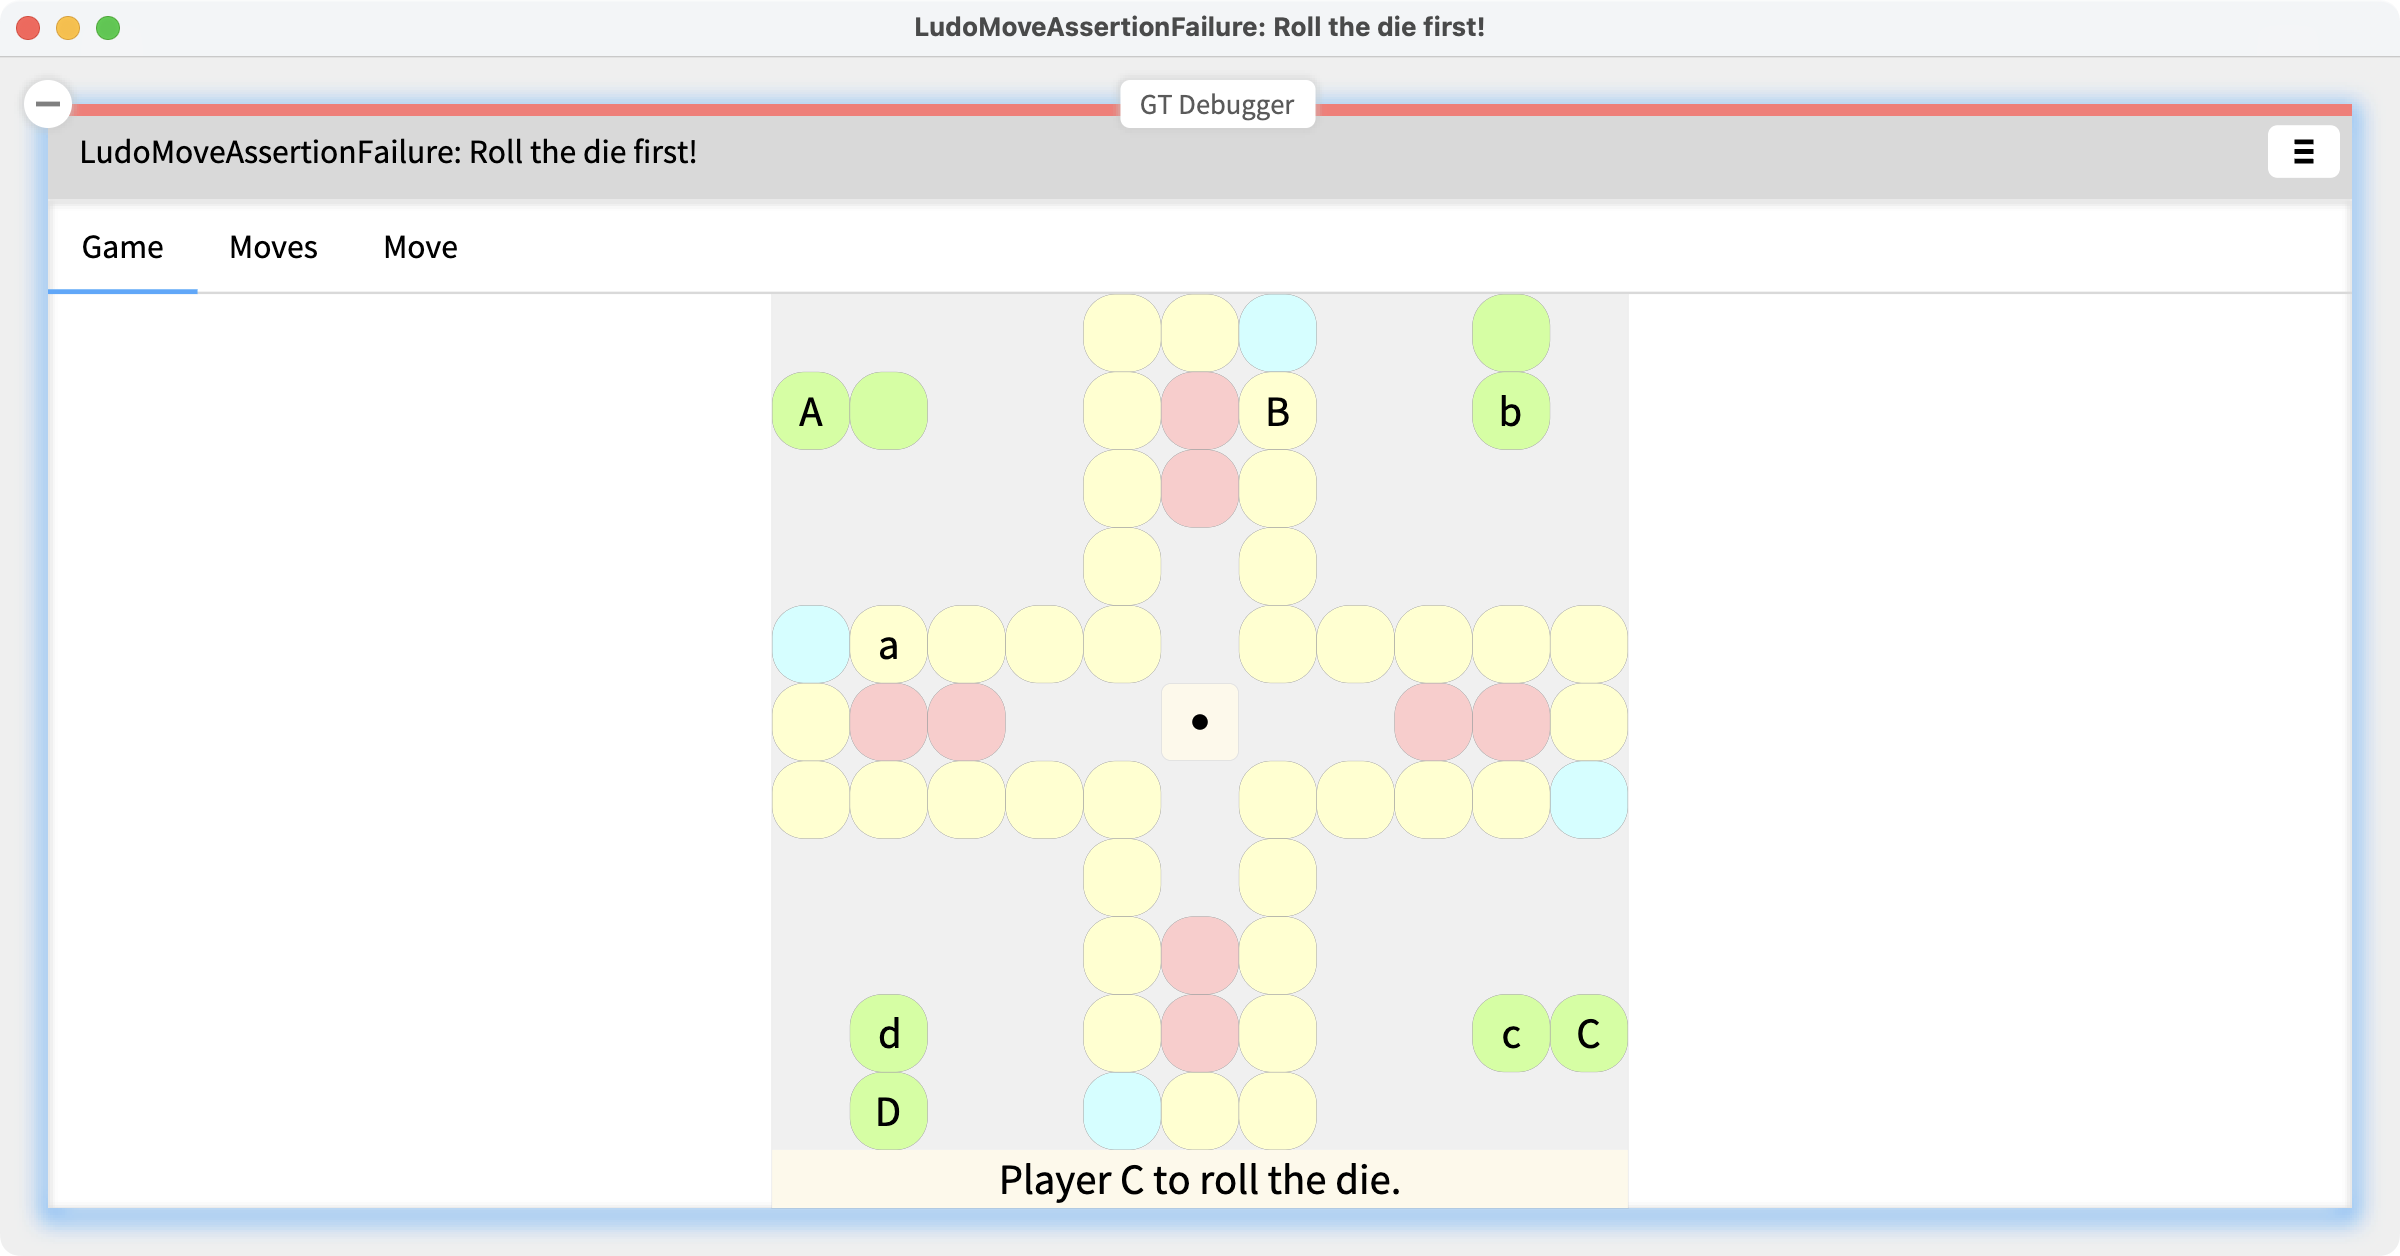
\includegraphics[width=\columnwidth]{ludoView1-Game}
  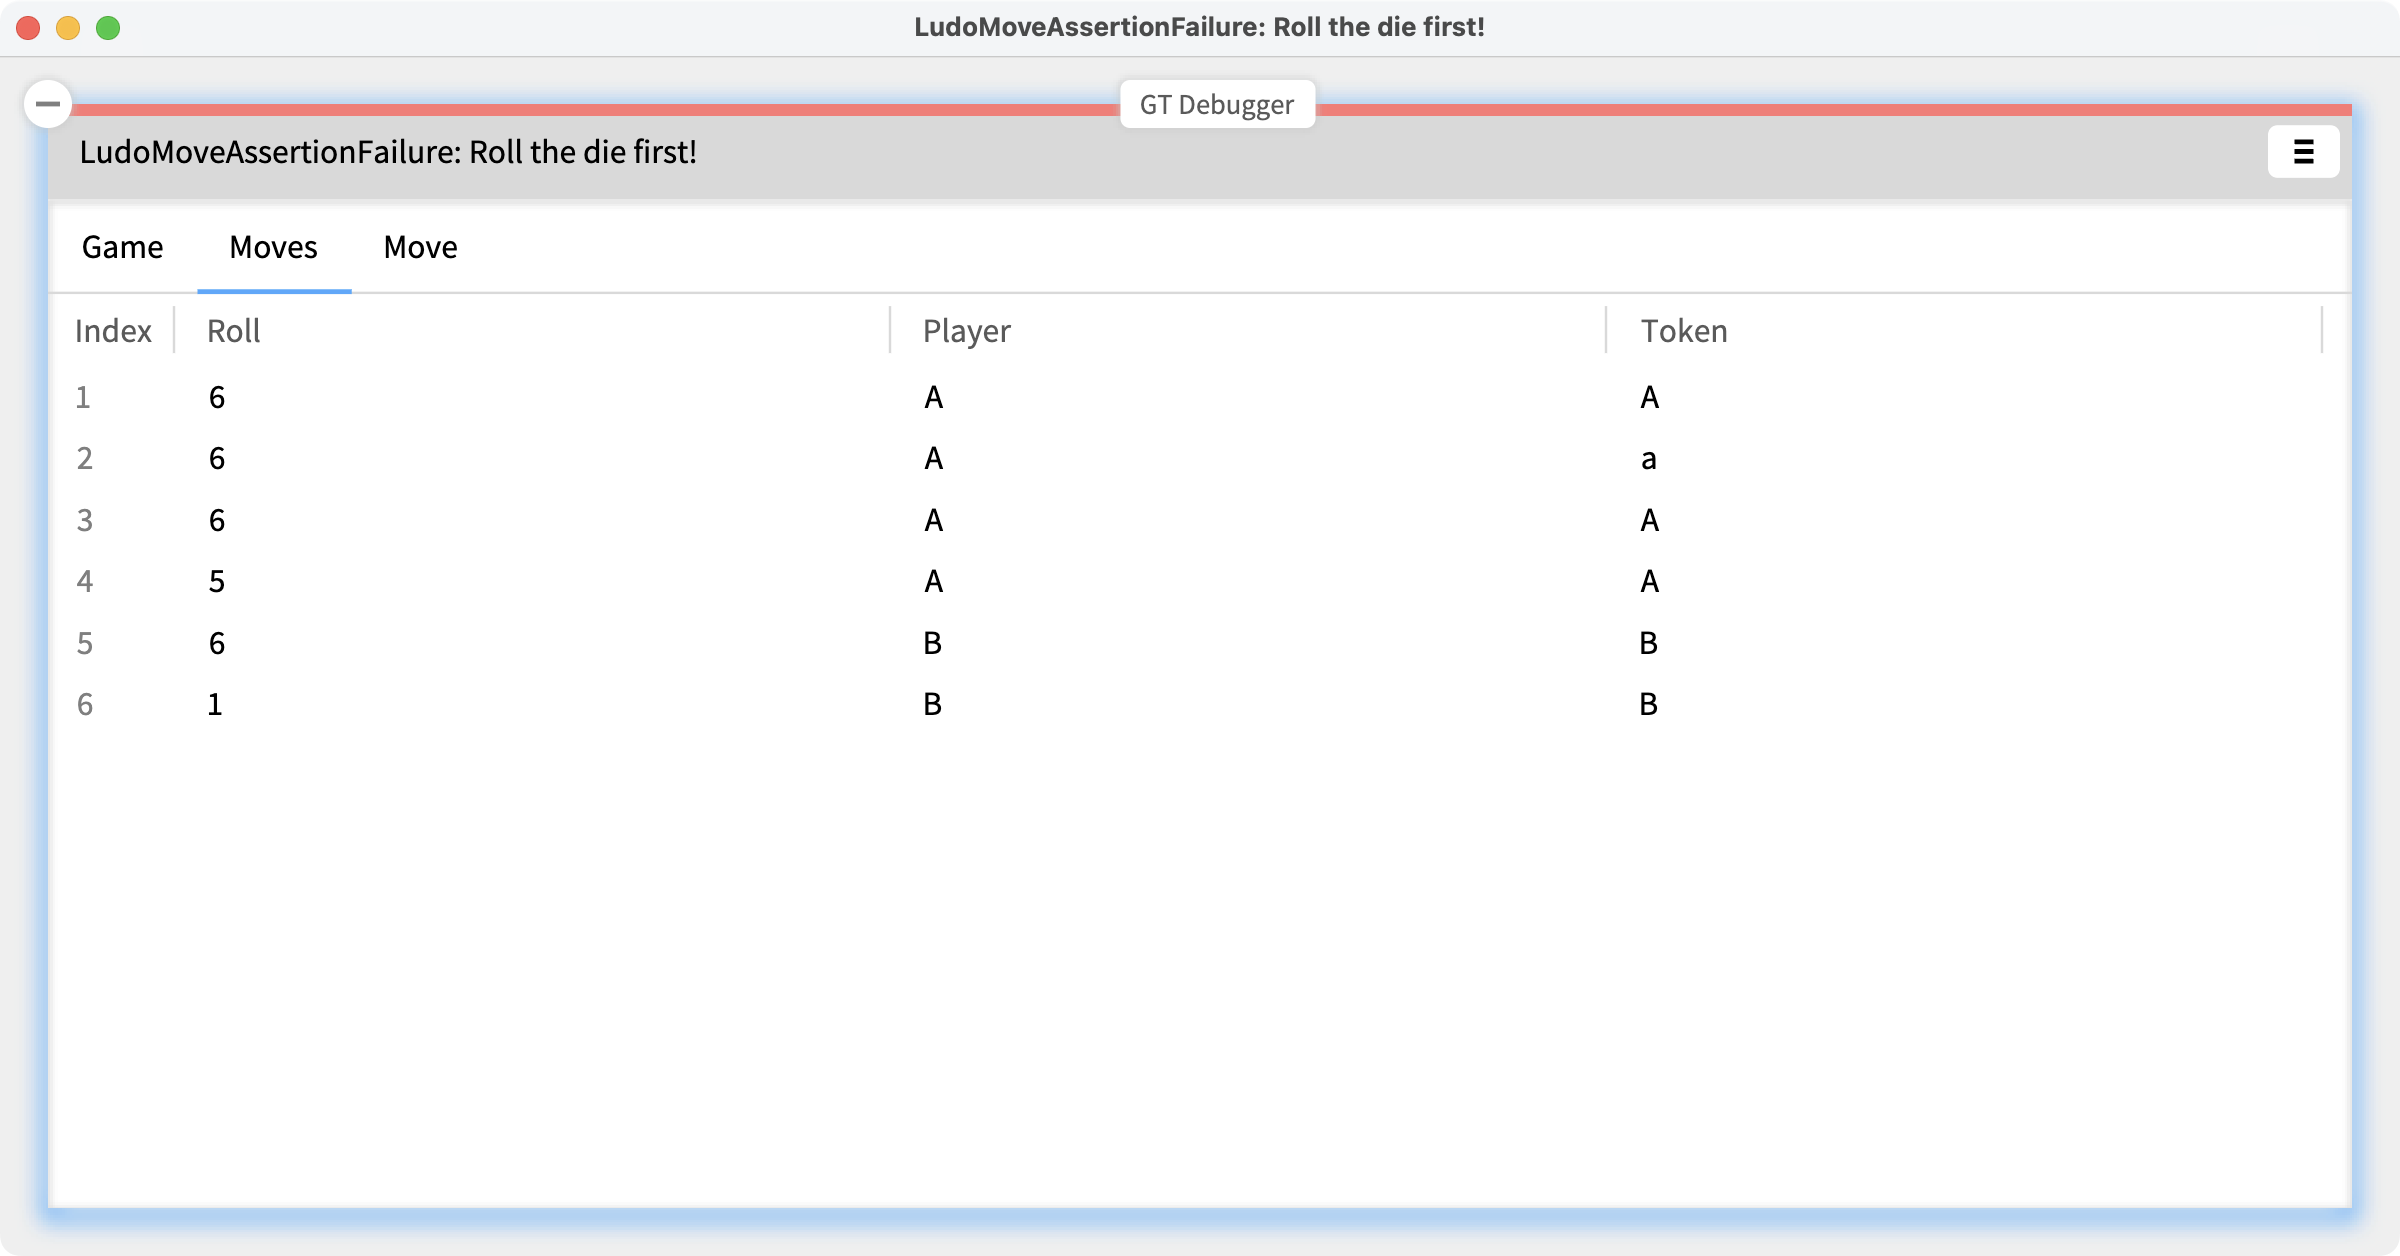
\includegraphics[width=\columnwidth]{ludoView2-Moves}
  \caption{Custom debugger views for the Ludo game.}
  \label{fig:ludoCustomViews}
\end{figure}

The assertion diff debugger view we saw earlier in \autoref{fig:stringComparisonView} is similarly defined as a method of \st{AssertionFailure}.
\begin{code}
gtTwoPanesStringDiffFor: aView
	<gtView>
	<gtExceptionDebuggingView>
	| assertionContext |
	self gtHasStack ifFalse: [ ^ aView empty ].
	assertionContext := self gtLocateAssertEqualsContextWithComparableTypes.
	assertionContext ifNil: [ ^ aView empty ].
	^ aView forward
		title: 'Textual Diff';
		priority: 0;
		object: [ assertionContext ];
		view: #gtTwoPanesStringDiffFor:
\end{code}
The key difference is that not every \st{AssertionFailure} is raised as the result of a string comparison.
For this reason, in lines $6-7$, the view will be suppressed (\st{^ aView empty}) in case the assertion did not fail in the context of an \st{assert:equals:} check.

% ============================================================
\section{Providing domain-specific debugger interactions}\label{sec:interactions}

The examples we have seen so far have reused existing inspector views

\todo{
Show the scripter example.
To test user interface interaction, we use a ``scripter'', that builds a GUI with labeled elements that react to events.
We can then check assertions about the state of the UI after these events.
The classic debugger is too low level.
Instead we can have a graph view of the hierarchy of scripter steps, showing the failed assertions.
This is done in AssertionFailure -- gtScripterStepsFor:
}

\st{AssertionFailure>>#gtScripterStepsFor:}

\todo{
Mention other domains from the moldable debugger, such as event-driven apps and parsers?
}

% ============================================================
\section{Enabling automated fixes}\label{sec:fixes}

\todo{
Introduce the deprecation special case.
Collector views.
Demo the empty view fix example.
Discuss the LifeWare tests?
}

% ============================================================
\section{Future directions}\label{sec:directions}

\todo{
Providing views with access to the debugger context.
Moldable exceptions for other platforms -- what do you need?
}

\ac{As a side note.
Technically we have access to the raised exception just when initially opening the debugger.
Any step over action for example could lead to another exception being raises.
The standard behaviour in Pharo is to always open the debugger on an exception.
The default one is OupsNullException, but also in case an exception was explicitly raised doing a step into for example, changes the exception to the default one.
I think we should more or less also do that.
Currently we never change the exception that was raised in the debugger, even if when stepping we get another one.
Just we can extend that with the notion of the last “real” exception that was raised, and a history of exceptions raised in that debugging session.
Like that we could have step actions/view added by an exception that can be use as long as another explicit exception was not raised.}

% ============================================================
\section{Related work}\label{sec:related}

\todo{Expand this list}

Moldable Debugger
\cite{Chis15c}

On the Dichotomy of Debugging Behavior Among Programmers
\cite{Bell18a}
Online developer survey shows that IDE-provided debuggers are not used as often as expected.

A Simple and Extensible Graphical Debugger
\cite{Hans97a}
An early example of an extensible debugger

Grammar-Driven Generation of Domain-Specific Language Debuggers
\cite{HuiW08a}
Generating debuggers for DSLs from the grammar spec.

Declaratively Defining Domain-Specific Language Debuggers
\cite{Lind11a}
Using a high-level spec to define DSL debuggers

Disciplined Exceptions
\cite{Meye88a}
First paper describing the use of exceptions in DbC.
\ac{
One argument reviewer B can bring :)), is that that exceptions are bad and should be avoided.
We can also emphasize that when working with frameworks having dedicated exceptions can help developers understand what is happening.
Users will not be exposed to exceptions, but developers need to reason about them.
And if they can help, developers can actually have a bigger incentive to create custom exceptions.}

% ============================================================
\section{Conclusion}\label{sec:conclusion}

\todo{xxx}


%% The acknowledgments section is defined using the "acks" environment
%% (and NOT an unnumbered section).
%\begin{acks}
%To Robert, for the bagels and explaining CMYK and color spaces.
%\end{acks}

\bibliographystyle{ACM-Reference-Format}
\bibliography{moldableExceptions}


\end{document}
\endinput

